Debido a las necesidades del presente proyecto, se optó por la utilización de una comunicación en serie asíncrona de tipo half-duplex bajo el estándar RS-232 con una configuración de trama 115200/8N1. Las características de dicha comunicación entre dispositivos se detallan a continuación:
\par
\paragraph*{Comunicación serie}
    La comunicación serie o serial transmite un único bit a la vez de forma secuencial, es decir, un bit tras otro, uno a la vez. Aunque es más lenta que una comunicación paralela, tiene la ventaja de que físicamente requiere de una sola conexión (un solo cable). Además, tiene un límite de distancia mucho mayor frente a una comunicación en paralelo.
    \par
    \paragraph*{Asíncrona}
En la comunicación asíncrona, la sincronización se restablece con la transmisión de cada carácter mediante el uso de bits de inicio y parada que, dependiendo de la tecnología utilizada, puede haber 1, 1,5 o 2 bits de parada.
\par
\paragraph*{Half-Duplex}
 De manera similar, cuando dos dispositivos de comunicación de datos se comunican en un entorno Half-Duplex, un dispositivo debe ser el transmisor y el otro el receptor. Para permitir la comunicación bidireccional, periódicamente tienen que invertir roles.    
 \par
 \paragraph*{Estándar RS-232}
La sección de características eléctricas del estándar RS-232 incluye especificaciones sobre los niveles de tensión, tasa de cambio de niveles de las señales e impedancia de la línea. El estándar RS-232 original se definió en 1962, previo a los días de la lógica TTL (Transistor-Transistor Logic), por lo que no es de extrañar que no utilice niveles lógicos de 5 voltios. En cambio, se define un nivel alto de salida con tensiones entre +5 y +15 voltios y un nivel bajo entre –5 y –15 voltios. Los niveles lógicos de entrada se definieron para proporcionar un margen de ruido de 2 voltios, por lo tanto un nivel alto para la entrada debe estar comprendido entre +3 a +15 voltios y un nivel bajo entre –3 a –15 voltios. En el actual proyecto, por incidencia directa del microcontrolador Atmega328, se emplearon salidas de +5V para niveles lógicos altos. 
\par
\paragraph*{Velocidad de transmisión}
    Indica el número de bits por segundo. En nuestro caso 115200 por defecto.
    \paragraph*{Trama 8n1}
    \par
    \paragraph*{El número de bits de datos}
    Refiere a la cantidad de bits (word) en la transmisión. En nuestro caso 8 bits.
    \par
    \paragraph*{El número de bits de stop}
    Utilizado para indicar el fin de la comunicación de un paquete. Mientras más bits de paro se usen, mayor será la tolerancia a la sincronía de los relojes de los dispositivos involucrados, sin embargo, la transmisión será más lenta. Para este proyecto se utilizó un bit de stop.
    \par
    \paragraph*{Y si cuenta con bit de paridad}
    El bit de paridad es una forma sencilla de verificar si hay errores en la transmisión serial. Para nuestro contexto no fue necesario definir bits de paridad, puesto que la complejidad de los datos enviados y recibidos no era elevada.
    \par
Finalmente para configurar, con las características mencionadas con anterioridad, la UART del microcontrolador Atmega328  se modificaron los registros correspondientes según la hoja de datos del fabricante y según la siguiente fórmula para determinar el registro de UART Baud Rate Register (UBRR0).
\begin{figure}[!htb]
  \begin{center}
    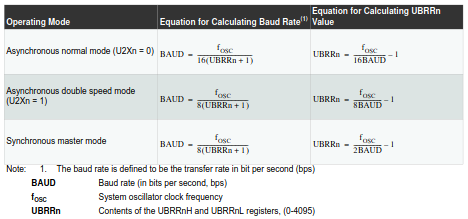
\includegraphics[width=0.92\textwidth]{imagenes/UARTbaudRateTable.png}
  \end{center}
  \caption{Tabla para calcular el registro de Baud Rate}
  \label{fig:baudRateTable}
\end{figure}
\FloatBarrier

